\chapter{Related Work}

\section{Retrieval Methodologies for Educational Content}
\label{sec:retrieval-methodologies}

Designing an effective search or question-answering system for educational settings requires adapting retrieval methodologies to the type of content involved, whether it be plain text such as lecture notes and transcripts, slides containing both text and figures, or video recordings of lectures. The current best practice favors a two-stage retrieval architecture that balances scalability with precision.

\subsection{Hybrid Sparse-Dense Retrieval for Text}
\label{subsec:hybrid-retrieval}

In the first stage, retrieval is broad and efficient, designed to quickly narrow down a large collection to a smaller candidate set. Hybrid sparse–dense retrieval has proven especially effective for text-heavy materials such as lecture transcripts, textbooks, or slide decks. In this approach, a sparse retriever such as BM25 or SPLADE is combined with a dense retriever such as a bi-encoder BERT or SciBERT. Sparse retrieval ensures that exact technical terms, formulas, or names are not overlooked, while dense retrieval provides semantic matching that can capture paraphrases or rewordings of concepts. For instance, a query about a ``photosynthesis diagram'' would benefit from sparse retrieval if the exact term appears in the document, while a dense retriever could still surface relevant passages describing plant energy processes even when phrased differently. Empirical evidence supports the robustness of the hybrid approach; Luan et al. (2021) demonstrated that combining sparse and dense signals yields superior performance over either method alone, particularly in scientific domains~\cite{luan2021sparse_dense}. To scale hybrid retrieval, efficient vector indices such as hierarchical navigable small-world (HNSW) graphs can be extended to support hybrid vectors or to efficiently merge results~\cite{lin2021densifying}. Many RAG systems for education adopt this hybrid method on a knowledge base of lessons or FAQs to ensure high recall.

\subsection{Multimodal Embeddings for Video Retrieval}
\label{subsec:multimodal-embeddings}

For video lectures or other multimodal content, dense retrieval based on multimodal embeddings is increasingly common. Models such as M2HF index video segments into dense vectors that encode visual frames, audio cues, and ASR transcript information~\cite{liu2022m2hf}. Text queries are mapped into the same embedding space, enabling cross-modal retrieval. This approach is advantageous over relying solely on transcript text, as it allows the retrieval of segments in which the visual modality is decisive—for example, locating ``the slide showing the cell cycle'' even when the transcript contains only a vague reference. The challenge of index size is addressed by segmenting videos into short windows, each represented by high-dimensional embeddings, and using approximate nearest neighbor search (e.g., FAISS or Annoy) to maintain efficiency. When transcripts or slide text are available, the hybrid sparse--dense approach introduced in Section~\ref{subsec:hybrid-retrieval} can be extended to multimodal contexts: combining OCR-extracted text and captions with visual tags produces more effective retrieval than relying solely on dense visual features, as purely visual features are not easily expressed as sparse signals. In practice, educational video retrieval often relies on maintaining both dense indices for semantic matches and inverted indices for textual signals.

\subsection{Reranking and Query Adaptation}
\label{subsec:reranking-adaptation}

Query adaptation constitutes an important dimension for specialized educational queries. For specialized educational queries, preprocessing or expansion may be required. For example, mathematical queries may be normalized by converting LaTeX into textual equivalents to ensure matches across both formats. LLMs can also be used to generate paraphrases of queries or, more experimentally, to produce synthetic images from text queries that can serve as additional search modalities. Although still exploratory, such query-driven modality augmentation holds promise for educational scenarios, such as automatically generating diagrams from student questions to facilitate diagram-based retrieval.

In the second stage, reranking is applied to the top candidates—typically the top 50 or 100—using slower but more precise methods. Cross-attentional rerankers, often based on transformer models such as BERT, take both the query and the candidate as input and compute a joint relevance score. This approach captures subtle distinctions that bi-encoder methods miss, such as differentiating between “a slide that mentions photosynthesis” and “a slide that explains photosynthesis in detail.” While computationally expensive, reranking remains feasible at this stage since only a limited number of candidates are evaluated. Multimodal cross-attentional rerankers further enrich this process by incorporating visual or layout information alongside text.

More recently, LLM-based reranking has emerged as a promising paradigm. Instead of relying on a fixed, pre-trained reranker, a multimodal LLM can be prompted to evaluate the relevance of retrieved passages directly or to synthesize an answer using retrieved evidence. For instance, DynamicRAG uses outputs from an LLM as feedback for reranking in a RAG pipeline, dynamically adjusting which passages to keep~\cite{sun2025dynamicrag}. Similarly, in a MRAG setup, more advanced relevancy measures have been proposed to better select which images, captions, or text to feed to the LLM, thereby reducing noise in the context~\cite{mortaheb2025reranking}. Such methods blur the line between retrieval and generation, providing both reranking and contextualized responses, and have been increasingly applied to educational chatbots and tutoring systems.

In practice, educational retrieval pipelines combine these methods to maximize performance. A typical system might retrieve textbook passages through hybrid retrieval, video segments through multimodal dense retrieval, and then rerank all candidates using either a cross-attentional model or a multimodal LLM. This two-stage strategy has become the prevailing standard because it delivers an effective balance between recall in the first stage and precision in the final ranking, thereby ensuring that the retrieved answers are both comprehensive and contextually relevant.


\section{Educational applications}

\subsection{Multimodal Retrieval}

To support evaluation and foster progress in multimodal retrieval for educational applications, researchers have assembled several new datasets that capture the multimodal nature of academic content. Between 2023 and 2025, multiple benchmarks have been introduced to reflect the diversity of lecture materials, textbooks, and visually rich documents.  
The Lecture Presentations Multimodal (LPM) dataset, released at ICCV 2023, is a notable example~\cite{lee2023lpm}. It contains approximately 180 hours of lecture videos delivered by ten lecturers across multiple subjects, aligned with more than 9,000 lecture slides. The dataset provides high-quality annotations linking slide content, including both figures and text, with corresponding speech segments. LPM defines three tasks that are directly relevant to education: figure-to-text retrieval, where a figure from a slide must be matched to the appropriate spoken segment; text-to-figure retrieval, where a segment of lecture speech or transcript is used to identify the relevant illustrative figure; and the generation of slide explanations. Baselines and human performance have been reported, and even fine-tuned vision–language models encountered significant difficulty on these tasks. This dataset has already inspired follow-up work, such as PolyViLT, which seeks to improve cross-modal alignment between slides and speech.

Another dataset is CK-12 Textbook QA (CK12-QA), which, although originally designed for question answering, doubles as a testbed for retrieval-augmented reasoning. Alawwad et al. (2025) propose a multimodal document ranking and retrieval supervision method for CK12-QA, showing that RAG significantly helps when retrieving both text and diagrams from lessons~\cite{alawwad2025jetrtqa}. Their findings revealed that retrieval substantially improves reasoning performance, though challenges remain, particularly in aligning question references with the correct diagram.

Beyond these examples, additional academic lecture video datasets have been introduced. The M\(^3\)AV dataset (ACL 2024) comprises 367 hours of university lectures in computer science, mathematics, and medicine, with transcripts and OCR-extracted slide text, including mathematical formulas, aligned with the videos~\cite{chen2024m3av}. Although M\(^3\)AV emphasizes recognition tasks such as ASR and slide generation, it provides rich multimodal data that can be repurposed for retrieval research. Earlier resources, such as lecture collections from VideoLectures.NET, contained smaller-scale alignments of subtitles and slides, but LPM and M\(^3\)AV substantially scale up both the size and the quality of annotations, enabling more rigorous evaluations of lecture segment retrieval.

Another relevant area involves benchmarks for visually rich document retrieval. The Jina-VDR (Visually Rich Document Retrieval) benchmark suite was introduced alongside Jina-Embeddings-v4, covering multimodal and multilingual document types (charts, tables, scanned pages, etc.)~\cite{guenther2025jinaembeddingsv4}. Improved performance on these tasks directly translates into more effective educational resource search, such as retrieving the precise slide containing a particular chart referenced in a query.

General-purpose cross-modal retrieval benchmarks also continue to play a role. Datasets such as MSR-VTT, MSVD, LSMDC, Flickr30k, and COCO provide open-domain evaluation tasks, while BEIR and MTEB offer text-focused retrieval suites. For example, the M\(^3\)HF model reported strong results on MSR-VTT, MSVD, DiDeMo, and ActivityNet Captions, demonstrating robustness across popular video–text retrieval benchmarks. More recently, the introduction of M-BEIR extended BEIR into multimodal domains, offering a broad evaluation suite that includes both text-only and cross-modal retrieval tasks. This extension has been adopted in the training of models such as MM-Embed, which benefits from exposure to multiple retrieval domains, some of which share similarities with educational materials.

In summary, the ecosystem of benchmarks has rapidly expanded to reflect educational scenarios, including lecture alignment datasets such as LPM, textbook-based reasoning datasets such as CK12-QA, and visually rich document retrieval datasets such as Jina-VDR. Nevertheless, important gaps remain. In particular, a large-scale benchmark for within-video moment retrieval in lecture recordings designed to locate the exact timestamp at which a given concept is explained has yet to be developed. As multimodal applications in education continue to grow, it is likely that the research community will address these gaps by creating more task-specific datasets.

\subsection{Modality Fusion}
  
A central challenge in multimodal retrieval is determining how to effectively fuse information from different modalities. The choice of fusion strategy whether early fusion, late fusion, or a hybrid approach directly influences the quality of the learned embeddings and the effectiveness of the retriever. Recent work has explored these strategies through multi-stage pipelines that aim to capture both coarse- and fine-grained alignments across modalities.

Early fusion, or feature-level fusion, merges modalities prior to computing similarity. This approach yields joint representations that more richly encode cross-modal interactions. For example, the M2HF model for video retrieval combines CLIP-based visual features with audio features to generate audio-guided visual representations that highlight sound-producing regions within frames, and fuses motion features derived from optical flow with visual features to emphasize movement. In this way, a video segment can be embedded as a single vector capturing synchronized cues across modalities, which is particularly useful in lecture settings where spoken language, slide text, and gestures jointly define relevance.

Late fusion, or decision-level fusion, instead computes similarity scores separately for each modality and combines them at the output stage, typically through weighted score averaging or rank fusion. In an educational search context, a query may be matched independently against slide text and slide images, with the results subsequently aggregated. Late fusion offers robustness and modularity, as demonstrated by cases in which a keyword hit in the ASR transcript can elevate a candidate despite weak visual similarity. Many retrieval pipelines adopt late fusion as part of a two-stage process, where candidates are retrieved using one modality and reranked using a cross-modal model.

Hybrid fusion strategies have recently gained attention as they combine the strengths of both approaches. M2HF exemplifies such a design by performing early fusion within video streams (e.g., audio–visual and motion–visual) and then applying text–video retrieval at multiple levels, followed by late fusion of the resulting scores. This multi-level approach significantly improved recall across diverse video retrieval tasks and allowed M2HF to achieve strong performance on benchmarks such as MSR-VTT, MSVD, LSMDC, DiDeMo, and ActivityNet.

A further refinement is cross-attentional fusion, which departs from dual-encoder architectures that generate independent embeddings per modality. Instead, cross-encoder models compute direct attention between modalities and between query and item, enabling deep, token-level fusion. For example, the PolyViLT model ingests aligned slide text, figures, and speech transcripts and applies cross-attention with a multi-instance learning (MIL) loss to align slide figures with specific spoken segments~\cite{lee2023lpm}. By capturing these fine-grained many-to-many alignments such as a single spoken segment referring to one figure among many on a slide cross-attentional models outperform independent embedding methods for retrieval of figure–speech pairs. As discussed in Section~\ref{sec:retrieval-methodologies}, the computational cost of cross-attention makes such models impractical for large-scale first-stage retrieval, though they are highly effective in reranking top candidates. An important practical dimension of fusion is modality balancing, which ensures that no single modality dominates the relevance scoring process. Techniques such as modality-specific weighting and loss balancing are commonly used to achieve this. In M2HF, a multimodal balance loss was introduced to encourage the model to utilize audio and motion signals alongside visual cues. This balancing is essential in educational contexts for instance, in mathematics lectures, transcripts may not explicitly describe the content of diagrams, making the visual modality indispensable for accurate retrieval.

\subsection{NotebookLM}

NotebookLM is an AI-powered note-taking and research assistant developed by Google Labs\footnote{\url{https://blog.google/technology/ai/notebooklm-google-ai/}}, built on the Gemini family of models\footnote{\url{https://deepmind.google/technologies/gemini/}}. Designed to synthesize information from user-uploaded materials, the system emphasizes grounded responses, multimodal comprehension, and support for research workflows. While NotebookLM is marketed as a general-purpose productivity tool, its capabilities overlap with multimodal educational assistants such as our proposed system for HCMUT lectures.

NotebookLM supports diverse input formats, including PDF documents, Google Docs, Google Slides, Microsoft Word (.docx), PowerPoint presentations (.pptx), web URLs, YouTube links, EPUB files, CSV files, Google Sheets, markdown files, and images with OCR capabilities \footnote{\url{https://notebooklm.google.com/get-started}}. The system performs structured ingestion and can interpret textual content as well as visual elements such as tables, diagrams, and slide images. Recent updates introduce advanced multimodal reasoning, enabling comprehensive question answering based on charts, graphs, images, diagrams, video transcripts, and mathematical content, with improved support for computational and technical reasoning \footnote{\url{https://blog.google/technology/google-labs/notebooklm-updates/}}.

This multimodal capability aligns with academic materials that combine formulas, diagrams, and spoken explanations. However, NotebookLM treats uploaded materials as isolated documents rather than components of a structured pedagogical sequence, limiting its effectiveness for course-level organization.

NotebookLM employs RAG to ensure responses are grounded in uploaded documents rather than solely in parametric model memory \cite{lewis2020rag}. When answering a query, the system retrieves relevant text segments and conditions generation on them, frequently accompanied by inline citations that reference specific sections of the source material. This reduces hallucinations and supports academic verification \footnote{\url{https://blog.google/technology/ai/notebooklm-citations/}}.

\begin{figure}[H]
    \centering
    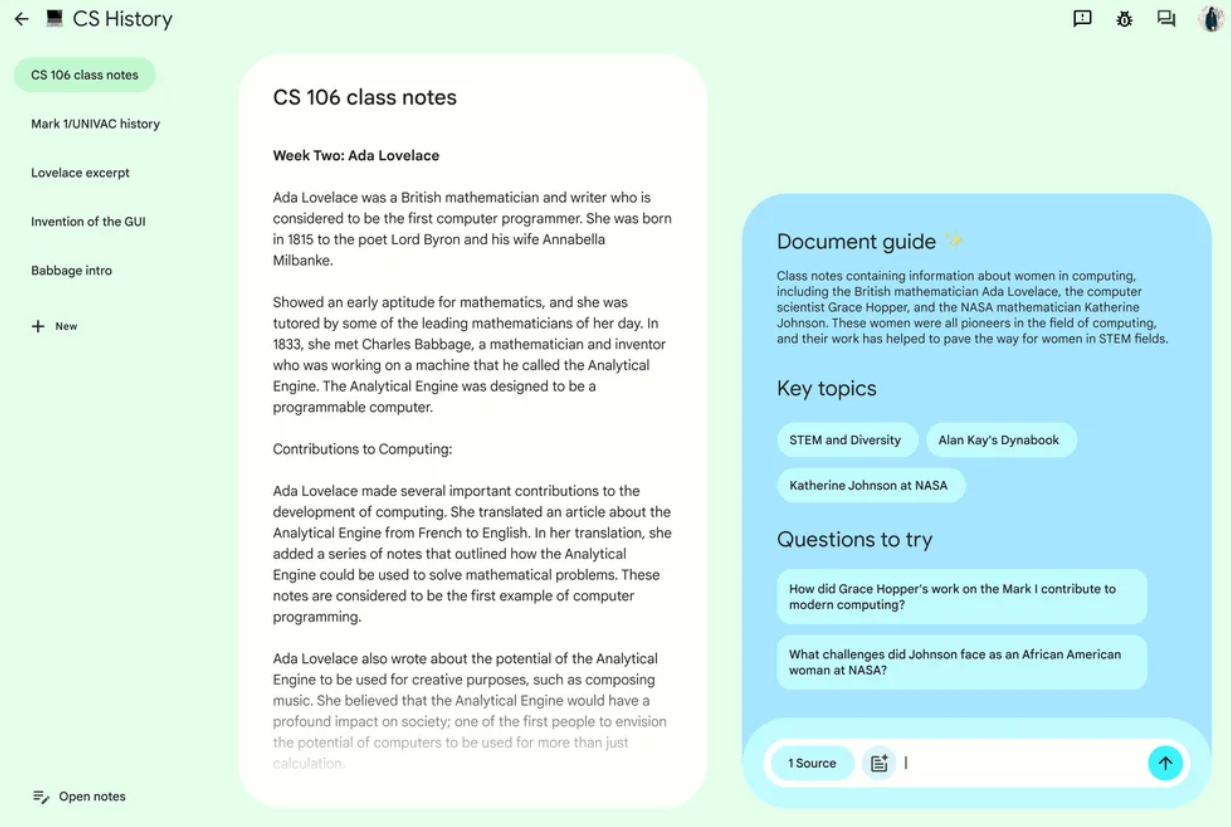
\includegraphics[width=0.9\textwidth]{img/pdz/11-notebooklm.png}
    \caption[NotebookLM]{NotebookLM}
    \label{fig:NotebookLM}
\end{figure}

Despite this grounding, complex analytical tasks such as mathematical reasoning, algorithm evaluation, or code execution may still rely on internal model reasoning and can produce incorrect interpretations without external validation layers. The NotebookLM interface is shown in Figure~\ref{fig:NotebookLM}\footnote{\url{https://blog.google/technology/ai/notebooklm-google-ai/}}.

Beyond static summarization and Q\&A, NotebookLM introduces several learning-focused features:

\begin{itemize}
    \item Structured document summaries \footnote{\url{https://blog.google/technology/ai/notebooklm-summaries/}},
    \item AI-generated flashcards and quizzes for active recall \footnote{\url{https://blog.google/technology/ai/notebooklm-learning-tools/}},
    \item Podcast-style audio overviews generated from uploaded materials \footnote{\url{https://blog.google/technology/ai/notebooklm-audio-overviews/}},
    \item Narrated visual summaries similar to lecture recap videos \footnote{\url{https://blog.google/technology/ai/notebooklm-audio-overviews/}}
\end{itemize}

These features support multiple learning modalities (reading, listening, reviewing). However, generated study resources depend on document completeness and may not capture contextual elements conveyed verbally during lectures.


NotebookLM enforces privacy by not using uploaded materials for model training and storing sources privately unless shared \footnote{\url{https://notebooklm.google.com/privacy}}. This makes the tool suitable for proprietary lecture materials. The system is deployed on both web and mobile platforms, supporting flexible access \footnote{\url{https://blog.google/technology/apps/notebooklm-mobile/}}.

In contrast, an institutional deployment such as our proposed system may require deeper integration with internal platforms, including lecture capture pipelines, LMS authentication, and course-specific permissions.


Although NotebookLM provides strong baseline functionality, several limitations motivate our specialized system:

\begin{table}[H]
\centering
\caption[NotebookLM Comparison]{Comparison between NotebookLM and our proposed system.}
\label{tab:comparison-notebooklm}
\begin{tabular*}{\textwidth}{@{\extracolsep{\fill}}p{0.45\textwidth}p{0.45\textwidth}@{}}
\toprule
\textbf{NotebookLM Design Focus} & \textbf{Opportunity for Our System} \\ \midrule
Manual document uploads & Automatic ingestion from slides, recordings, LMS \\
Document-centric representation & Course-aware structuring by lecture/week/topic \\
General-purpose technical reasoning & Domain-specific pedagogical sequencing and curriculum alignment \\
Generic responses without instructor oversight & Instructor feedback loops and domain-tuned prompting \\
Individual learning workflows & Institutional integration and cohort-based learning analytics \\ \bottomrule
\end{tabular*}
\end{table}

Thus, while NotebookLM is an excellent general-purpose multimodal research assistant optimized for individual learners and researchers, it is not designed for institutional deployment with curriculum-aware features. Our system (BK-MInD) aims to bridge this gap by providing structured course-centric knowledge modeling, pedagogically sequenced learning paths, institutional integration with LMS platforms, and automated ingestion of lecture materials—enabling end-to-end lecture understanding tailored to the needs of educational institutions.



\newpage